\chapter{Горизонты де Ситтера и космологическая вероятность}

\lectureoverview{Горизонт — это не просто причинная граница. Для стационарного наблюдателя это тепловая система: термометр, удерживаемый на собственном расстоянии \(\rho\) от горизонта, показывает температуру порядка \(1/(2\pi\rho)\), тогда как гравитационное красное смещение делает излучение, наблюдаемое вдали, гораздо более холодным. Мы перенесем этот урок о черных дырах в пространство де Ситтера, выведем фиксированный радиус горизонта \(H^{-1}\) и запишем метрику статической области наблюдателя. Во второй половине лекции термодинамика доводится до ее тревожных следствий: конечная энтропия де Ситтера, возвраты Пуанкаре, больцмановские мозги, вечная инфляция и проблема меры. В заключительном обсуждении точные суперсимметричные структуры теории струн отделяются от все еще неизвестной схемы, которая могла бы описывать наш мир.}

\section{Что означает, что горизонт горячий}

Мы начинаем до формальной лекции с вопроса, который задает направление всему вечеру.

\begin{classroomqa}
\audiencequestion{У космологического горизонта нет черной дыры. За счет какого механизма он тем не менее может быть горячим?\lecturetimestamp{00:00:17}}
\lecturerresponse{Механизм тот же, что и у горизонта черной дыры. Полезно поставить вопрос операционально: что показывает термометр, удерживаемый вблизи горизонта, и какое излучение достигает наблюдателя далеко от него?}
\end{classroomqa}

Первый опыт локален. Пусть термометр удерживается на фиксированном собственном расстоянии \(\rho\) от любого гладкого неэкстремального горизонта. Достаточно близко к горизонту геометрия принимает универсальную риндлеровскую форму, и термометр показывает
\begin{equation}
T_{\rm local}(\rho)\simeq \frac{1}{2\pi\rho}
\label{eq:l09-local-temperature}
\end{equation}
в единицах, где \(\hbar=c=k_B=1\). При восстановлении констант получаем
\begin{equation}
k_B T_{\rm local}(\rho)\simeq \frac{\hbar c}{2\pi\rho}.
\end{equation}
Расходимость при \(\rho\to0\) не означает, что падающий наблюдатель сталкивается с обычной материальной печью. Это температура, приписываемая наблюдателем, который остается неподвижным прямо вне горизонта и потому должен ускоряться всё сильнее.

Вступительный разговор также разводит три понятия, которые легко смешать: энергию, температуру и энтропию.

\begin{classroomqa}
\audiencequestion{Если посылать фотоны в черную дыру, измерим ли мы по-прежнему ту же энтропию, или изменяется только энергия?\lecturetimestamp{00:01:22}}
\lecturerresponse{Как только фотон становится недоступным за горизонтом, дополнительная информация оказывается скрытой. В упрощенном битовом языке, используемом здесь, один фотон может скрыть один дополнительный бит и тем самым увеличить энтропию. Энергия, температура и энтропия связаны, но они не взаимозаменяемы.}
\end{classroomqa}

\editorialnote{Для физической черной дыры изменение энтропии термодинамически задается соотношением \(dS=dE/T_H\); это не универсально один бит на фотон независимо от его энергии. Утверждение об одном бите — информационно-теоретическая идеализация лекции.}

Пригоризонтная область непрерывно испускает и вновь поглощает высокочастотные квантовые флуктуации. Для стационарного наблюдателя горизонт придает этим флуктуациям тепловой характер. Но это сразу порождает загадку. Если область сколь угодно горяча, почему далекого наблюдателя не ослепляют фотоны со сколь угодно большой энергией?

\section{Красное смещение и температура Хокинга}

Обычная горячая стена остается источником высокочастотного излучения, даже когда мы стоим далеко от нее. Горизонт отличается тем, что его излучению приходится подниматься, претерпевая гравитационное красное смещение. Скорость фотона остается \(c\); уменьшается его энергия,
\begin{equation}
E=\hbar\omega,
\qquad
\omega_{\rm received}<\omega_{\rm emitted}.
\end{equation}
Аналогия с кусочком мела, использованная в лекции, полезна лишь до этого места. Брошенный камень, поднимаясь, замедляется, тогда как фотон продолжает двигаться со скоростью света, а его частота и энергия уменьшаются.

Для шварцшильдовской черной дыры температура, измеряемая наблюдателем на бесконечности, равна
\begin{equation}
T_H=\frac{1}{8\pi M}
\label{eq:l09-hawking-natural}
\end{equation}
в единицах \(G_N=\hbar=c=k_B=1\). В обычных единицах,
\begin{equation}
T_H=\frac{\hbar c^3}{8\pi G_N M k_B}.
\label{eq:l09-hawking-full}
\end{equation}

\begin{figure}[htbp]
\centering
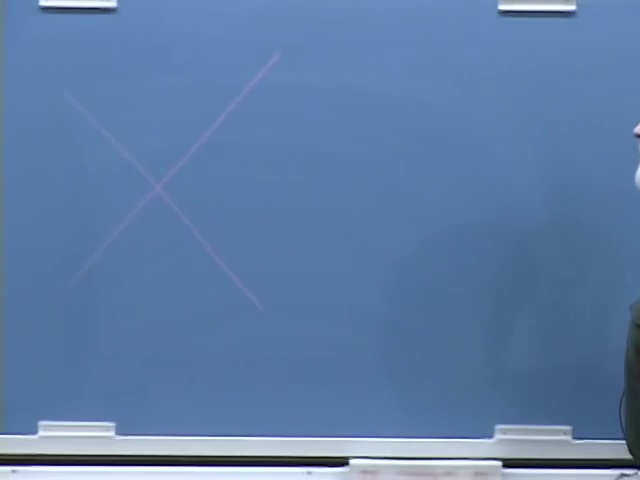
\includegraphics[width=0.68\textwidth]{lecture_09_figure_02.png}
\caption{Температура Хокинга \(T_H=1/(8\pi M)\) в естественных единицах.}
\lectureframe{00:08:12}
\end{figure}

Чем больше черная дыра, тем она холоднее. В лекции это объясняют, прослеживая назад типичный фотон. У тепловых фотонов характерная энергия \(E_\gamma\sim T_H\). Фотон, достигающий бесконечности с энергией порядка \(M^{-1}\), когда он возникает вблизи горизонта, имеет гораздо большую локальную энергию. Красное смещение между пригоризонтным слоем и бесконечностью сильнее для большей дыры, поэтому асимптотическая температура оказывается ниже.

\begin{classroomqa}
\audiencequestion{Если шварцшильдовское время замирает на горизонте, не следует ли нам прослеживать фотон, который изначально упал внутрь и увеличил массу дыры?\lecturetimestamp{00:04:19}}
\lecturerresponse{Для вопроса о температуре надо прослеживать фотоны, испускаемые наружу. Они начинаются с очень высокой локальной частоты, теряют энергию, выбираясь наружу, и приходят как излучение Хокинга. Судьба исходного падающего фотона — отдельный вопрос об информации.}
\end{classroomqa}

\section{Планковский слой и растянутый горизонт}

Насколько близко к горизонту можно доверять локальному соотношению из уравнения~\eqref{eq:l09-local-temperature}? В лекции планковская длина принимается за наименьшее осмысленное расстояние в полуклассическом описании. Это подсказывает наличие тонкого слоя примерно в одну планковскую длину снаружи от математического горизонта, заполненного флуктуациями планковского масштаба. Он непрерывно испускает и поглощает.

Большинство испущенных квантов не уходит. Лишь те, что направлены в очень узкий конус наружу, избегают падения обратно. Кванты, испущенные под произвольными углами, возвращаются к горизонту. Исходящие и входящие возбуждения сталкиваются, порождая пары и другие частицы; в этом смысле стационарное описание содержит тонкий слой чрезвычайно горячего вещества.

\begin{figure}[htbp]
\centering
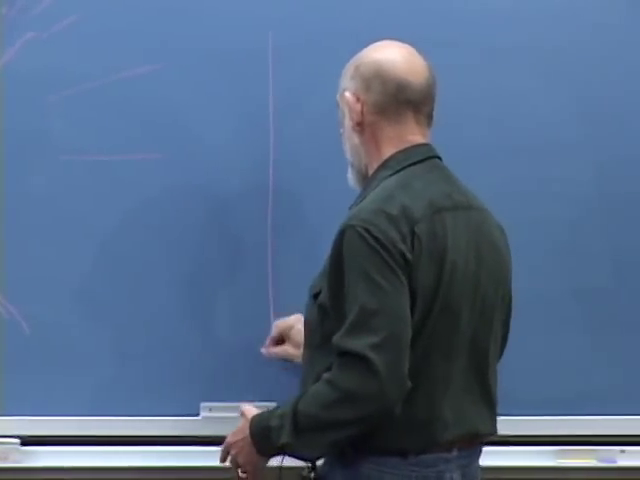
\includegraphics[width=0.74\textwidth]{lecture_09_figure_03.png}
\caption{Узкий конус выхода для пригоризонтного излучения. Большинство локально испущенных квантов возвращается к горизонту.}
\lectureframe{00:11:38}
\end{figure}

Существует и дополняющая пространственно-временная картина. Вдали от горизонта виртуальную флуктуацию можно схематически представить короткой замкнутой петлей: возбуждение частица–античастица возникает и исчезает прежде, чем оно сможет стать асимптотическим состоянием. Вблизи горизонта флуктуация может лежать по обе стороны причинной границы. Для внешнего наблюдателя внешняя часть выглядит как частица, испущенная горизонтом и позднее вновь поглощенная. Очень малая доля уходит и становится излучением Хокинга.

\begin{classroomqa}
\audiencequestion{На внешней диаграмме такая флуктуация простирается от \(t=-\infty\) до \(t=+\infty\)?\lecturetimestamp{00:15:00}}
\lecturerresponse{Точное классическое положение горизонта приводит к такому кажущемуся сингулярным описанию. На практике мы заменяем его растянутым горизонтом, времениподобной поверхностью примерно в одну планковскую длину снаружи. Тогда испускание и повторное поглощение происходят при конечных внешних временах.}
\end{classroomqa}

\begin{figure}[htbp]
\centering
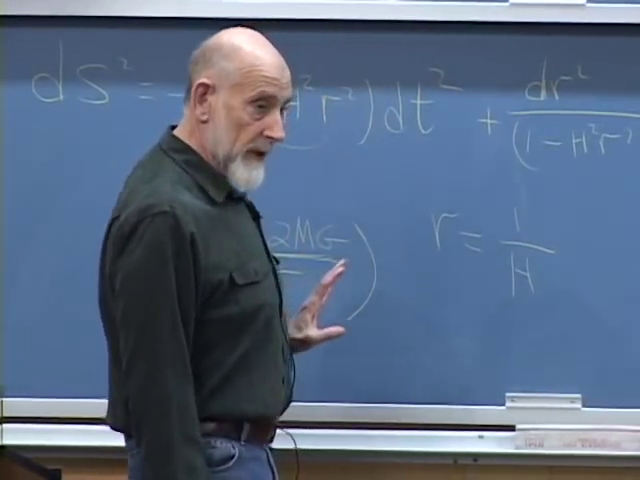
\includegraphics[width=0.72\textwidth]{lecture_09_figure_04.png}
\caption{Классический горизонт и расположенный рядом растянутый горизонт, используемый во внешнем описании.}
\lectureframe{00:15:52}
\end{figure}

Растянутый горизонт не является новой инвариантной границей. Это эффективная поверхность, помещаемая туда, где полуклассическая геометрия перестает быть надежной. Квантовые флуктуации материи и самой геометрии размывают точное положение на планковских масштабах. Эта конструкция сводит неопределенность к поверхности, на которой внешнее описание остается конечным.

В этом локальном рассуждении ничто не различает, принадлежит ли горизонт черной дыре или ускоренно расширяющейся Вселенной. Это и есть мост к пространству де Ситтера.

\section{Пространство де Ситтера в расширяющихся координатах}

Формальная лекция начинается с пространственно-плоского слоения пространства-времени де Ситтера,
\begin{equation}
ds^2=-dt^2+e^{2Ht}d\mathbf{x}^2,
\qquad
d\mathbf{x}^2=dx^2+dy^2+dz^2.
\label{eq:l09-flat-slicing}
\end{equation}
Константа \(H\) задает скорость расширения де Ситтера. Множитель появляется как \(e^{2Ht}\), потому что метрика измеряет квадрат расстояния; фиксированный координатный интервал имеет физическую длину
\begin{equation}
D(t)=e^{Ht}\lvert\Delta\mathbf{x}\rvert.
\end{equation}

\begin{figure}[htbp]
\centering
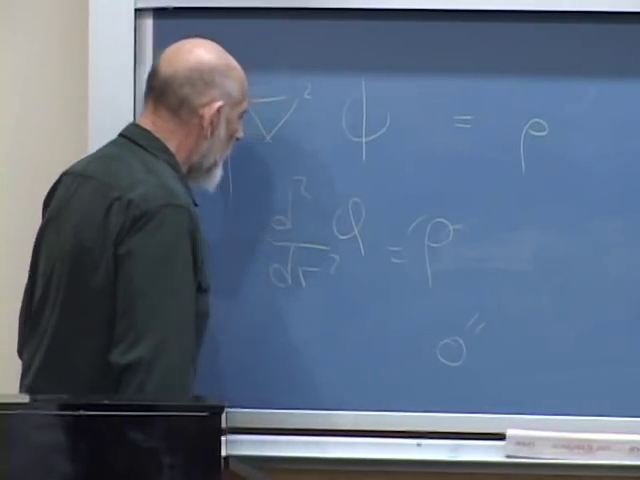
\includegraphics[width=0.78\textwidth]{lecture_09_figure_05.png}
\caption{Экспоненциально расширяющаяся метрика де Ситтера в плоских координатах.}
\lectureframe{00:18:50}
\end{figure}

Эти координаты наглядно показывают расширение, но помещают будущую бесконечность бесконечно далеко вверх по странице. Чтобы перенести ее на доску, введем конформное время
\begin{equation}
\eta=-\frac{1}{H}e^{-Ht},
\qquad
-\infty<\eta<0.
\label{eq:l09-conformal-time}
\end{equation}
Тогда
\begin{equation}
dt=\frac{d\eta}{-H\eta},
\qquad
e^{Ht}=-\frac{1}{H\eta},
\end{equation}
и уравнение~\eqref{eq:l09-flat-slicing} принимает вид
\begin{equation}
ds^2=\frac{1}{H^2\eta^2}
\left(-d\eta^2+d\mathbf{x}^2\right).
\label{eq:l09-conformal-metric}
\end{equation}
При \(t\to+\infty\) имеем \(\eta\to0^{-}\). Бесконечное собственное время сжато в конечную горизонтальную линию \(\eta=0\).

\editorialnote{Преобразование времени по ходу записи на доске несколько раз исправляется. Уравнение~\eqref{eq:l09-conformal-time} дает согласованную форму: раннее космическое время отображается в \(\eta\to-\infty\), а будущая бесконечность — в \(\eta\to0^{-}\).}

\begin{figure}[htbp]
\centering
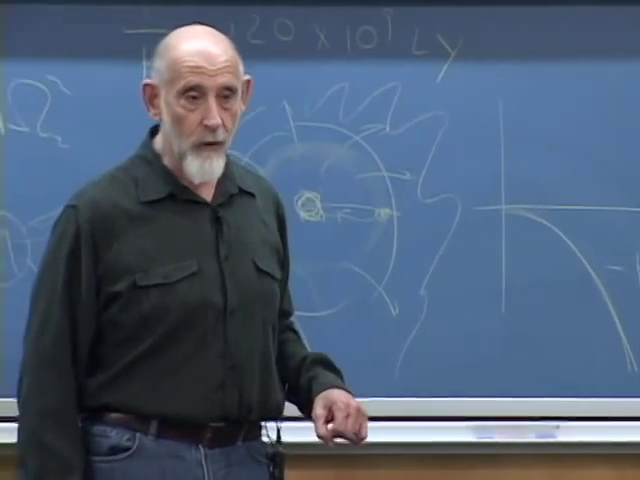
\includegraphics[width=0.82\textwidth]{lecture_09_figure_06.png}
\caption{Преобразование к конформному времени и конформно-плоская метрика.}
\lectureframe{00:21:24}
\end{figure}

Конформный множитель умножает и временной, и пространственный члены, поэтому не изменяет светоподобные направления. Для радиального светового луча,
\begin{equation}
ds^2=0
\quad\Longrightarrow\quad
-d\eta^2+dx^2=0
\quad\Longrightarrow\quad
\frac{dx}{d\eta}=\pm1.
\label{eq:l09-null-rays}
\end{equation}
Следовательно, на конформной диаграмме свет идет под углом \(45^\circ\). Поэтому смена координат полезна: причинная достижимость становится видимой.

\section{Причинная область одного наблюдателя}

Представьте наблюдателя, мировая линия которого продолжается в течение бесконечного собственного времени. На компактифицированной диаграмме она оканчивается в одной точке на \(\eta=0\). Любой сигнал, который он вообще может получить, лежит внутри обратного светового конуса этой конечной точки. События вне этого конуса никогда не могут послать ему сигнал, сколько бы он ни ждал.

\begin{figure}[htbp]
\centering
\includegraphics[width=0.78\textwidth]{lecture_09_figure_07.png}
\caption{Предельный обратный световой конус наблюдателя в конформных координатах де Ситтера.}
\lectureframe{00:24:38}
\end{figure}

У второго наблюдателя другой конус. Эти две доступные области перекрываются, но ни одна не охватывает все пространство-время. В дальнейшем мы примем точку зрения первого и будем называть этот обратный световой конус каузальной областью наблюдателя.

На рисунке кажется, будто область сжимается по направлению к будущему, но координатная ширина не есть собственное расстояние. На срезе при постоянном \(\eta\) квадрат физического расстояния между наблюдателем в точке \(x=0\) и горизонтом в точке \(x=\Delta x\) равен
\begin{equation}
D^2=\frac{(\Delta x)^2}{H^2\eta^2}.
\label{eq:l09-horizon-distance-start}
\end{equation}
Горизонт — нулевая линия под углом \(45^\circ\), оканчивающаяся при \(\eta=0\), поэтому
\begin{equation}
\Delta x=\lvert\eta\rvert.
\end{equation}
Подстановка дает
\begin{equation}
D_{\rm hor}^2=\frac{1}{H^2},
\qquad
D_{\rm hor}=\frac{1}{H}.
\label{eq:l09-horizon-radius}
\end{equation}
Координатное расстояние уменьшается, но конформный множитель растет ровно настолько, чтобы это скомпенсировать. Собственный радиус горизонта постоянен.

\begin{figure}[htbp]
\centering
\includegraphics[width=0.80\textwidth]{lecture_09_figure_08.png}
\caption{Вывод на доске, переводящий сжимающийся координатный интервал в фиксированное собственное расстояние \(H^{-1}\).}
\lectureframe{00:28:42}
\end{figure}

\section{Статическая область}

Постоянный радиус горизонта подсказывает координаты, приспособленные к центральному наблюдателю. Не выводя преобразование координат, в лекции записывают результат:
\begin{equation}
ds^2=
-\left(1-H^2r^2\right)d\tau^2
+\frac{dr^2}{1-H^2r^2}
+r^2d\Omega_2^2.
\label{eq:l09-static-patch}
\end{equation}
Коэффициенты зависят от \(r\), а не от \(\tau\). Эта координатная карта покрывает статическую область наблюдателя,
\begin{equation}
0\le r<\frac{1}{H}.
\end{equation}

\begin{figure}[htbp]
\centering
\includegraphics[width=0.88\textwidth]{lecture_09_figure_09.png}
\caption{Метрика статической области де Ситтера и ее сравнение с фактором Шварцшильда.}
\lectureframe{00:34:22}
\end{figure}

Сходство со Шварцшильдом видно сразу:
\begin{equation}
f_{\rm dS}(r)=1-H^2r^2,
\qquad
f_{\rm Schw}(r)=1-\frac{2G_NM}{r}.
\end{equation}
В обоих случаях горизонт в статических координатах находится там, где \(f(r)=0\). Для де Ситтера
\begin{equation}
1-H^2r^2=0
\quad\Longrightarrow\quad
r_H=H^{-1}.
\end{equation}
Здесь карта сингулярна, точно так же как координаты Шварцшильда сингулярны на горизонте черной дыры. Тем не менее глобальные геометрии различаются важным образом. Наблюдатель у черной дыры находится снаружи и смотрит внутрь; наблюдатель де Ситтера находится внутри и смотрит наружу.

\begin{classroomqa}
\audiencequestion{Как геометрия может быть статической, если свободно отпущенные частицы расходятся в экспоненциально расширяющейся Вселенной?\lecturetimestamp{00:36:06}}
\lecturerresponse{Статичность не означает, что каждая частица остается неподвижной. Это означает, что коэффициенты метрики и результат повторного эксперимента не зависят от момента начала. Отпустите сейчас две частицы — и они начнут ускоренно расходиться; повторите тот же эксперимент позже — и произойдет то же самое движение.}
\end{classroomqa}

\begin{classroomqa}
\audiencequestion{Наблюдают ли две расходящиеся частицы красное смещение друг друга?\lecturetimestamp{00:38:34}}
\lecturerresponse{Да. Их возрастающее разделение вызывает относительное красное смещение, хотя метрика, приспособленная к наблюдателю, не зависит от времени.}
\end{classroomqa}

\section{Температура, наблюдаемая изнутри}

Пригоризонтные структуры пространства Шварцшильда и де-ситтеровского пространства локально эквивалентны. Поэтому горизонт де Ситтера испускает и вновь поглощает тепловые кванты. Редкий фотон распространяется внутрь, к центральному наблюдателю, теряя энергию при подъеме по потенциалу статической области. Измеряемая в центре температура Гиббонса--Хокинга равна
\begin{equation}
T_{\rm dS}=\frac{H}{2\pi}
\label{eq:l09-de-sitter-temperature}
\end{equation}
в естественных единицах. Неподвижный термометр на радиусе \(r\) показывает значение с толмановским красным смещением
\begin{equation}
T_{\rm local}(r)=
\frac{T_{\rm dS}}{\sqrt{1-H^2r^2}},
\label{eq:l09-tolman}
\end{equation}
которое расходится при \(r\to H^{-1}\) и вблизи горизонта сводится к уравнению~\eqref{eq:l09-local-temperature}.

\editorialnote{В лекции масштаб получают из расстояния до горизонта и красного смещения, а не выписывают явно уравнения~\eqref{eq:l09-de-sitter-temperature} и \eqref{eq:l09-tolman}. Здесь указана стандартная нормировка этого рассуждения.}

Для наблюдаемого позднего ускорения в лекции используется оценка периода
\begin{equation}
H^{-1}\sim 20\times10^9\ {\rm light\ years}.
\label{eq:l09-lecture-horizon-estimate}
\end{equation}
Тогда типичный фотон горизонта имеет длину волны, сравнимую с миллиардами световых лет. Это не реликтовое микроволновое излучение; оно несравненно холоднее.

Операциональный мысленный эксперимент — это удочка космологического масштаба. Алиса остается при \(r=0\), прикрепляет термометр к очень длинному тросу, по которому также передаются данные, и позволяет космическому отталкиванию унести прибор наружу. Она останавливает его чуть не доходя до горизонта, ждет возвращения сигнала и обнаруживает большую локальную температуру. Термометр рядом с ней в центре показывает крошечное значение \(H/(2\pi)\). Один и тот же горизонт допускает оба показания, потому что они снимаются при разных гравитационных потенциалах.

\section{Пересечение горизонта}

Классическое внешнее описание напоминает знакомую историю с черной дырой. Боб в центре наблюдает, как Алиса удаляется. Ее сигналы испытывают все большее красное смещение и приходят все медленнее; она кажется распластанной по горизонту и в конце концов гаснет. Более поздняя путешественница, Джейн, выглядит как еще один, более тонкий слой в осадочной стопке у границы.

\begin{classroomqa}
\audiencequestion{С нашей точки зрения, проходят ли объекты вообще через космологический горизонт?\lecturetimestamp{00:45:30}}
\lecturerresponse{Не в классическом описании статического наблюдателя. Их сигналы краснеют и затухают, тогда как их видимое положение приближается к горизонту. Однако в их собственном свободнопадающем описании они пересекают его, не встречая локально сингулярной поверхности.}
\end{classroomqa}

\begin{classroomqa}
\audiencequestion{Горизонт горяч только для наблюдателей, которые остаются поблизости, не пересекая его? Падающий наблюдатель ведь не поджаривается просто от того, что проходит через него, верно?\lecturetimestamp{00:48:27}}
\lecturerresponse{В своей системе отсчета Алиса пересекает его гладко. Экстремальная температура относится к стационарному описанию. Если Боб настаивает на том, чтобы разрешать Алису все ближе к горизонту, ему приходится облучать ее все более короткими длинами волн. Такая попытка построить гейзенберговский микроскоп тогда вносит достаточно энергии, чтобы поджарить то, что он пытается наблюдать.}
\end{classroomqa}

Это не противоречие между двумя локальными событиями. Стационарный наблюдатель и падающий используют радикально разные измерения. Комплементарность горизонта ставит вопрос о том, как оба описания могут быть верны, не позволяя одному наблюдателю напрямую сравнить дублированную информацию.

\section{Ньютоновская модель отталкивания вакуума}

В этот момент студент спрашивает, что заменяет гравитационный колодец черной дыры. Сасскинд отвечает, строя ньютоновскую модель. Пусть \(\phi\) — гравитационный потенциал, так что ускорение пробной частицы равно
\begin{equation}
\mathbf{a}=-\boldsymbol{\nabla}\phi.
\end{equation}
Для обычного нерелятивистского вещества уравнение Пуассона имеет вид
\begin{equation}
\nabla^2\phi=4\pi G_N\rho.
\label{eq:l09-poisson}
\end{equation}

\begin{classroomqa}
\audiencequestion{Если эффекты черной дыры связаны с ее гравитационным колодцем, что служит соответствующим источником в пространстве де Ситтера?\lecturetimestamp{00:49:36}}
\lecturerresponse{Сама энергия вакуума дает пространственно однородный гравитационный источник. В ньютоновском описании она создает квадратичный потенциал, а не колодец вида \(1/r\).}
\end{classroomqa}

\begin{figure}[htbp]
\centering
\includegraphics[width=0.78\textwidth]{lecture_09_figure_10.png}
\caption{Уравнение Пуассона и схематическая радиальная форма второй производной, используемая в лекции.}
\lectureframe{00:51:38}
\end{figure}

На доске опускаются нормировка, члены сферической меры, давление и поначалу даже общий знак, так что упражнение сводится к
\begin{equation}
\frac{d^2\phi}{dr^2}\sim H^2.
\end{equation}
Существенный вывод состоит в том, что постоянный источник дает квадратичную функцию. При знаке, требуемом отталкиванием де Ситтера,
\begin{equation}
\phi_{\rm dS}(r)=-\frac{1}{2}H^2r^2,
\qquad
a_r=-\frac{d\phi_{\rm dS}}{dr}=H^2r.
\label{eq:l09-de-sitter-potential}
\end{equation}
Ускорение направлено наружу и растет линейно с расстоянием. Решение уравнения \(\ddot r=H^2r\) дает
\begin{equation}
r(\tau)=A e^{H\tau}+B e^{-H\tau},
\end{equation}
так что растущая ветвь воспроизводит экспоненциальное расхождение.

\begin{figure}[htbp]
\centering
\includegraphics[width=0.76\textwidth]{lecture_09_figure_11.png}
\caption{Уравнение для однородного источника и квадратичный потенциал де Ситтера.}
\lectureframe{00:53:32}
\end{figure}

\editorialnote{В общей теории относительности слабополевое ускорение однородной жидкости зависит от \(\rho+3p\), а не только от \(\rho\). Для вакуумной энергии \(p=-\rho\), так что \(\rho+3p=-2\rho\) и ускорение является отталкивающим. Уравнение~\eqref{eq:l09-de-sitter-potential} дает правильно нормированный результат де Ситтера; вычисление на доске намеренно отслеживает только квадратичную зависимость и знак.}

Поместим в центр обычную массу \(M\). Тогда качественный потенциал принимает вид
\begin{equation}
\phi(r)=-\frac{G_NM}{r}-\frac{1}{2}H^2r^2,
\label{eq:l09-combined-potential}
\end{equation}
а радиальное ускорение равно
\begin{equation}
a_r=-\frac{G_NM}{r^2}+H^2r.
\end{equation}
При малых \(r\) побеждает локальное притяжение; при больших \(r\) побеждает вакуумное отталкивание. Их баланс достигается при
\begin{equation}
r_\ast=\left(\frac{G_NM}{H^2}\right)^{1/3}.
\label{eq:l09-turnaround}
\end{equation}
Это аккуратная версия максимума потенциала из лекции. Это качественно объясняет, почему близкие гравитационно связанные системы могут оставаться связанными, тогда как достаточно далекие галактики ускоренно удаляются.

\begin{figure}[htbp]
\centering
\includegraphics[width=0.78\textwidth]{lecture_09_figure_12.png}
\caption{Обычное притяжение вида \(1/r\) в сочетании с перевернутым квадратичным потенциалом де Ситтера.}
\lectureframe{00:58:20}
\end{figure}

\begin{classroomqa}
\audiencequestion{Обычные силы по-прежнему важны, или вакуумное отталкивание в конце концов разрывает всякий остров материи?\lecturetimestamp{00:57:29}}
\lecturerresponse{Нужно учитывать все силы. На достаточно малых масштабах доминируют электромагнитное связывание и локальная гравитация. Вакуумное отталкивание становится существенным лишь на огромных расстояниях, задаваемых \(H^{-1}\) и масштабом равновесия, соответствующим данной связанной массе.}
\end{classroomqa}

\section{Один источник, несколько названий}

Теперь ненадолго остановимся на терминологии. В используемой модели энергия вакуума, космологическая постоянная и тёмная энергия — не три аддитивные субстанции. Это три описания одного и того же источника \(w=-1\). Можно говорить о постоянном члене в уравнении Эйнштейна, о лоренц-инвариантной плотности энергии вакуума или о компоненте, вызывающей ускорение на поздних временах.

\begin{classroomqa}
\audiencequestion{Присутствуют ли однородный ньютоновский источник и квантовая энергия вакуума одновременно как отдельные эффекты?\lecturetimestamp{00:59:14}}
\lecturerresponse{Нет. Однородная плотность — это ньютоновская модель того же самого источника. Энергия вакуума, космологическая постоянная и, в этой лекции, тёмная энергия обозначают одну физическую компоненту.}
\end{classroomqa}

\begin{classroomqa}
\audiencequestion{Имеет ли тогда одно и то же явление классическое описание и квантовое описание?\lecturetimestamp{01:00:32}}
\lecturerresponse{Его микроскопическое происхождение может быть квантово-механическим, подобно тому как часть массы электрона имеет квантовое происхождение. Как только эффективная плотность энергии известна, она входит в классические гравитационные уравнения как обычный источник. Окончательного происхождения наблюдаемого значения мы не знаем.}
\end{classroomqa}

В планковских единицах наблюдаемая плотность энергии вакуума чрезвычайно мала:
\begin{equation}
\rho_\Lambda\sim10^{-123}\rho_{\rm Pl},
\label{eq:l09-planck-smallness}
\end{equation}
с точностью до соглашения, используемого для планковской плотности. Именно это малое число и составляет проблему космологической постоянной. По той же причине горизонт так велик: в четырёх измерениях
\begin{equation}
H^2=\frac{8\pi G_N}{3}\rho_\Lambda,
\qquad
r_H=H^{-1}.
\end{equation}
Если бы \(H\) было больше, горизонт был бы меньше, температура де Ситтера в центре — выше, а отталкивающее ускорение \(H^2r\) — сильнее.

\begin{classroomqa}
\audiencequestion{Связана ли крошечная космологическая постоянная с постоянной Планка и квантовыми флуктуациями?\lecturetimestamp{01:03:27}}
\lecturerresponse{Наиболее ясное сравнение получается в безразмерных планковских единицах, где \(G_N=\hbar=c=1\). В этих единицах плотность вакуума примерно на \(123\) порядков величины меньше естественной планковской плотности. Объяснение этой иерархии — одна из центральных загадок фундаментальной физики.}
\end{classroomqa}

\begin{classroomqa}
\audiencequestion{Должна ли энергия вакуума быть в точности постоянной космологической постоянной? Может ли ускоряющая компонента уменьшаться и в конце концов установиться на нуле?\lecturetimestamp{01:04:52}}
\lecturerresponse{Это логически возможная альтернатива: динамическое поле тёмной энергии могло бы изменяться со временем. В лекции принимается случай постоянной не потому, что все альтернативы были доказаны невозможными, а потому, что доступные на тот момент наблюдения всё сильнее указывали на поведение, близкое к космологической постоянной.}
\end{classroomqa}

\section{Астрономия в далёком будущем}

В асимптотически де-ситтеровской вселенной структуры, не связанные гравитационно, в конце концов пересекают горизонт наблюдателя. Космическое микроволновое фоновое излучение из-за красного смещения уходит ниже порога обнаружения. Далёкие галактики исчезают. Уцелевший астроном может видеть лишь слившийся локальный гравитационный остров внутри в остальном тёмной области.

\begin{classroomqa}
\audiencequestion{Без телескопа кто-нибудь вообще заметил бы, что далёкие галактики исчезли?\lecturetimestamp{01:06:17}}
\lecturerresponse{Вероятно, нет. Серьёзная проблема глубже: даже при наличии развитых приборов у будущих наблюдателей может не оказаться далёких трассеров и микроволнового фона, по которым мы сегодня делаем вывод о расширении.}
\end{classroomqa}

Тогда старая картина «островной вселенной» могла бы показаться убедительной. Парадокс Ольберса не заставил бы прийти к иному выводу, потому что он предполагает бесконечную, статическую, однородную совокупность светящихся источников; будущий наблюдатель видел бы лишь конечное число звёзд локального острова. Тёмная энергия не создаёт непрерывно новые галактики из пустого пространства взамен исчезнувших.

В точном пространстве де Ситтера горизонт не сжимается вокруг локальной галактики. Его физический радиус остаётся равным \(H^{-1}\), что неизмеримо больше размера галактики. Исчезает же несвязанная материя, уносимая за эту фиксированную причинную границу.

\begin{classroomqa}
\audiencequestion{Могли бы звёзды, выброшенные из галактики, служить пробными телами для обнаружения крупномасштабной геометрии?\lecturetimestamp{01:11:25}}
\lecturerresponse{Некоторое время — да. Выброшенные объекты и световые сигналы на больших базах могли бы зондировать геометрию. Но эффект становится заметным лишь на расстояниях порядка значительной доли миллиарда световых лет, так что эксперимент занял бы космологическое время.}
\end{classroomqa}

\begin{classroomqa}
\audiencequestion{Откуда мы знаем, что далёкий горизонт уже не скрыл от нас большую часть вселенной?\lecturetimestamp{01:11:45}}
\lecturerresponse{Мы уже видим достаточно много галактик, красных смещений и фонового излучения, чтобы измерить расширение и восстановить крупномасштабную геометрию. Будущие наблюдатели, лишённые этих трассеров, столкнулись бы с намного более трудной задачей вывода.}
\end{classroomqa}

\begin{classroomqa}
\audiencequestion{Если бы горизонт лежал сразу за Андромедой, было бы его присутствие очевидно?\lecturetimestamp{01:12:19}}
\lecturerresponse{Да. Такой маленький горизонт потребовал бы гораздо большего \(H\), и возникающее отталкивание сильно изменило бы движение Андромеды. Измеренное значение, напротив, помещает асимптотический горизонт на несравненно больший масштаб.}
\end{classroomqa}

\begin{classroomqa}
\audiencequestion{Могут ли за нашим горизонтом происходить новые Большие взрывы?\lecturetimestamp{01:13:25}}
\lecturerresponse{События за горизонтом не видны ни нам, ни нашим потомкам. Родственная, но более точная возможность — нуклеация пузырей при вечной инфляции — будет рассмотрена позже в лекции.}
\end{classroomqa}

Имея ракеты, часы и несколько миллиардов лет, будущие наблюдатели могли бы отправить исследователей через значительную часть этой области и восстановить её метрику. Однако на обычных лабораторных или цивилизационных масштабах времени этот эффект почти недоступен. Это различие поправляет слишком сильное утверждение, будто расширение было бы невозможно обнаружить: оно операционально труднодоступно, а не запрещено в принципе.

\begin{classroomqa}
\audiencequestion{Могли бы будущие исследователи определить геометрию гораздо раньше, не дожидаясь теплового возврата?\lecturetimestamp{01:21:40}}
\lecturerresponse{Безусловно. Возврат не является предлагаемым измерением. Исследователи, обмениваясь световыми сигналами на базах в миллиарды световых лет, могли бы построить карту статического патча за несравненно более короткое, хотя всё же космологическое, время.}
\end{classroomqa}

\begin{classroomqa}
\audiencequestion{Стерло бы красное смещение всю информацию, возвращённую такими исследователями?\lecturetimestamp{01:23:24}}
\lecturerresponse{Нет, если они зондируют масштабы, лежащие далеко внутри горизонта. База порядка миллиарда световых лет уже чувствительна к расширению и при этом даёт лишь умеренное красное смещение. Эксперимент ограничен главным образом своей огромной длительностью.}
\end{classroomqa}

\section{Конечная энтропия и возврат}

В термодинамическом смысле статический патч не пуст. Его горизонт характеризуется площадью
\begin{equation}
A_H=4\pi H^{-2},
\end{equation}
температурой \(T_{\rm dS}=H/(2\pi)\) и энтропией
\begin{equation}
S_{\rm dS}=\frac{A_H}{4G_N}
=\frac{\pi}{G_NH^2}
\label{eq:l09-de-sitter-entropy}
\end{equation}
в единицах \(\hbar=c=k_B=1\). Энтропия конечна. Поэтому статический патч, с должной осторожностью, можно представлять как тепловую полость с конечной энтропией, возбуждения которой в стационарном описании сосредоточены вблизи горизонта.

Обычный ящик с газом в равновесии на коротких временах кажется лишённым особенностей, но статистическая механика не запрещает флуктуаций. Если макросостояние имеет дефицит энтропии \(\Delta S\) по сравнению с равновесием, его вероятность примерно равна
\begin{equation}
P\sim e^{-\Delta S}.
\label{eq:l09-fluctuation-probability}
\end{equation}
Соответствующее время ожидания растёт как
\begin{equation}
t\sim t_0 e^{\Delta S}.
\end{equation}
Для конечной системы время возвращения в состояние, сколь угодно близкое к более раннему, есть время возврата Пуанкаре,
\begin{equation}
t_{\rm rec}\sim H^{-1}e^{S_{\rm dS}}.
\label{eq:l09-recurrence}
\end{equation}
Поскольку \(S_{\rm dS}\) для нашего горизонта имеет порядок \(10^{120}\), в лекции этот масштаб кратко записывается как \(e^{10^{120}}\). Измеряется ли префактор в годах, хаббловских временах или микроскопических единицах, это несущественно по сравнению с двойной экспонентой.

\begin{figure}[htbp]
\centering
\includegraphics[width=0.76\textwidth]{lecture_09_figure_13.png}
\caption{Обсуждение возврата; на доске — огромный экспоненциальный масштаб времени ожидания.}
\lectureframe{01:16:24}
\end{figure}

До такого возврата меньшие флуктуации встречаются несравненно чаще. Все молекулы в комнате могли бы собраться в одном углу; мог бы ненадолго образоваться сложный вихрь; в шутливой иерархии лекции тепловое движение могло бы собрать слона. Чем меньше требуемый дефицит энтропии, тем дешевле флуктуация.

\begin{classroomqa}
\audiencequestion{Являются ли возвраты Пуанкаре именно следствием квантовой механики?\lecturetimestamp{01:25:44}}
\lecturerresponse{Нет. Возвраты и редкие флуктуации возникают уже в классической статистической механике. Их применение к пространству де Ситтера использует нашу нынешнюю физическую картину, которая когда-нибудь может быть пересмотрена, но термодинамика и статистические рассуждения — одни из самых надёжных известных нам структур.}
\end{classroomqa}

Само значение вероятности в будущей теории может обрести более глубокий смысл. Susskind этого не отрицает. Его более узкий тезис состоит в том, что отказ от статистической механики лишь потому, что ее следствия на больших временах странны, означал бы отбросить один из лучше всего проверенных структурирующих принципов физики.

\section{Мозги Больцмана и типичные наблюдатели}

Предположим, что тепловая флуктуация создает целое состояние, подобное Большому взрыву. Это требует огромного уменьшения энтропии. Флуктуация, создающая одну солнечную систему, менее затратна; уже теплая Земля обходится еще дешевле. Если требуется лишь один наблюдатель, то наименее затратная флуктуация могла бы создать только функционирующий мозг с кажущимися воспоминаниями. Такого гипотетического наблюдателя называют мозгом Больцмана.

Проблема не в том, логически ли возможна одна странная флуктуация. Проблема в том, предсказывает ли космологическая модель, что почти каждый наблюдатель является именно такой флуктуацией. Мы рассуждаем, исходя из наших наблюдений, предполагая, что не являемся фантастически нетипичными. Теория, в которой обычные наблюдатели со связными космическими историями экспоненциально уступают по численности изолированным тепловым мозгам, подрывает такой вывод.

Поэтому проблема мозгов Больцмана — это количественная проверка на согласованность. Сравнивают ожидаемую численность обычных наблюдателей с численностью наблюдателей, порожденных флуктуациями. Если преобладают последние, то либо вакуум должен распасться прежде, чем они начнут возникать в огромном количестве, либо нужно изменить меру, либо следует пересмотреть космологические предположения.

Более ранний вопрос об ультрафиолетово--инфракрасной связи здесь явно откладывается. Аргумент о рекуррентности не зависит от разрешения этого отдельного вопроса.

\section{Вечная инфляция и пузырьковые вселенные}

Далее в лекции, не пытаясь дать полный вывод, вводится вторая вероятностная проблема. В метастабильном вакууме де Ситтера может нуклеироваться пузырь, в котором энергия вакуума ниже. Стенка пузыря расширяется, а его внутренняя область может развиться в открытую вселенную Фридмана--Робертсона--Уокера. Тем временем окружающая инфлирующая область продолжает расширяться и нуклеирует новые пузыри.

\begin{figure}[htbp]
\centering
\includegraphics[width=0.74\textwidth]{lecture_09_figure_14.png}
\caption{Пузырь с меньшей энергией вакуума, изображенный внутри инфлирующего фона де Ситтера.}
\lectureframe{01:29:38}
\end{figure}

Ключевая особенность состоит в экспоненциальном росте числа областей. Новый физический объем возникает быстрее, чем его поглощают пузыри, так что число пузырьковых областей растет без границ. Разные пузыри могут перейти в разные низкоэнергетические состояния и потому проявлять разную эффективную физику.

Чтобы выявить статистическую трудность, Susskind сначала отходит от космологии и рассматривает экспоненциально растущую человеческую популяцию с конечными, но неизвестными ресурсами. Предположим, что наблюдатели типичны среди всех людей за все время существования популяции. Если население удваивается в каждом поколении, а затем заканчивается, то половина всех людей живет в последнем поколении, три четверти — в двух последних, а семь восьмых — в трех последних:
\begin{equation}
f_n=1-2^{-n}.
\label{eq:l09-last-generations}
\end{equation}
Тогда предположение о типичности помещало бы нас неприятно близко к концу, хотя об общем запасе ресурсов нам ничего не известно. Это предлагается не как надежное предсказание вымирания человечества. Это предупреждение о том, что при экспоненциальном росте результат подсчета определяется отсечкой.

Пример с подбрасыванием монеты яснее формулирует обычное предположение о типичности. Если много экспериментаторов каждый подбрасывает честную монету \(N\) раз, то подавляющее большинство получает
\begin{equation}
n_H=\frac{N}{2}+O(\sqrt{N}).
\end{equation}
Наблюдатель с экстремальным результатом должен прежде всего заподозрить плохую модель или плохую монету, а не без доказательств считать, что он находится в фантастически редком хвосте распределения. Космологическая вероятность опирается на то же интуитивное представление о типичности, но в бесконечной популяции ей нужен четко определенный способ подсчета.

\section{Граница Эшера и проблема меры}

Геометрическая аналогия Susskind — это работа M.\ C.\ Escher \emph{Circle Limit IV}, диск, замощенный ангелами и дьяволами, которые кажутся меньше по мере приближения к границе. В гиперболической геометрии, представленной на рисунке, эти фигуры эквивалентны; их кажущийся евклидов размер меняется только из-за проекции.

\begin{figure}[htbp]
\centering
\includegraphics[width=0.76\textwidth]{lecture_09_figure_15.png}
\caption{Нарисованный на доске суррогат экспоненциально размножающихся фигур Эшера у круговой границы.}
\lectureframe{01:37:54}
\end{figure}

Представьте, что у Эшера конечны время, чернила и терпение. У края он в конце концов останавливается, возможно оставляя некоторые фигуры незавершенными. Поскольку число фигур экспоненциально растет с гиперболическим радиусом, конечный внешний слой содержит фиксированную по порядку величины долю всех нарисованных фигур. Приблизительно половина может лежать в последнем слое, как бы далеко наружу ни сдвигали отсечку.

Теперь спросим об отношении числа ангелов к числу дьяволов. В идеальном бесконечном узоре симметрия подсказывает равенство один к одному. Однако при любом конечном подсчете немного иная граница может включить гораздо больше фигур одного типа. Поскольку большая часть подсчета сосредоточена у границы, малая деформация этой границы приводит к изменению ответа на величину порядка единицы.

\begin{figure}[htbp]
\centering
\includegraphics[width=0.76\textwidth]{lecture_09_figure_16.png}
\caption{Граница отсечки доминирует в подсчете в экспоненциально растущем узоре.}
\lectureframe{01:43:06}
\end{figure}

Та же неоднозначность возникает и в вечной инфляции. Подсчитайте синие и розовые пузырьковые вселенные до некоторой временной отсечки, а затем сдвиньте отсечку на более позднее время. Оба подсчета расходятся, и их отношение может чувствительно зависеть от того, что понимается под \emph{time} и как проведена поверхность отсечки. Вероятностная мера — это предписание, которое регуляризует бесконечную популяцию и извлекает относительные вероятности. То, что разные правдоподобные предписания не согласуются друг с другом, и есть проблема меры.

\begin{classroomqa}
\audiencequestion{Есть ли связь между этой проблемой отсечки и ренормализацией?\lecturetimestamp{01:45:43}}
\lecturerresponse{Есть аналогия. В квантовой теории поля вводят решетку или ультрафиолетовую отсечку, затем уточняют ее и ищут величины, нечувствительные к краевым деталям регуляризатора. Космологи надеются на столь же устойчивое извлечение относительных вероятностей из вечной инфляции, но в обсуждаемой здесь схеме пока нет столь же решающего предписания.}
\end{classroomqa}

Эту аналогию не следует преувеличивать. Ренормализация успешна, когда контролируемый поток выделяет наблюдаемые, не зависящие от регуляризатора. Проблема меры как раз и состоит в том, что аналогичные инвариантные вопросы и предельная процедура остаются неясными. Сказать, что, возможно, мы задаем неправильный вопрос, — не решение, пока не указан правильный.

\begin{classroomqa}
\audiencequestion{Является ли эта картина с пузырями тем же самым явлением, что и инфляция в ранней Вселенной?\lecturetimestamp{01:48:19}}
\lecturerresponse{Они тесно связаны. При вечной инфляции родительский фон продолжает инфлировать, в то время как внутренние области локальных пузырей проходят собственную космологическую эволюцию. Наша наблюдаемая Вселенная могла бы находиться внутри одной такой области.}
\end{classroomqa}

\section{Можно ли увидеть столкновения пузырей?}

При встрече двух пузырей их энергии вакуума не просто складываются. Области с разными вакуумными состояниями разделяет доменная стенка, и геометрия этой стенки определяет, что может наблюдать каждая из сторон. В зависимости от положения столкновения относительно нашего прошлого светового конуса его след может быть скрыт или видим.

\begin{classroomqa}
\audiencequestion{Что происходит при столкновении двух вакуумных пузырей?\lecturetimestamp{01:52:07}}
\lecturerresponse{Столкновение создает геометрию доменной стенки, поведение которой зависит от двух вакуумов и от натяжения стенки. При благоприятных причинных обстоятельствах возмущение может войти в нашу наблюдаемую область и оставить анизотропный след.}
\end{classroomqa}

В лекции обсуждается холодная область в космическом микроволновом фоне как возможный кандидат и указывается на поляризацию вокруг круговой особенности как на различающий признак. Это намеренно подается как возможность, а не как обнаружение. Убедительный сигнал столкновения был бы революционным, потому что дал бы прямое свидетельство в пользу существования соседних пузырьковых областей и сделал бы проблему меры экспериментально неотложной.

\begin{figure}[htbp]
\centering
\includegraphics[width=0.70\textwidth]{lecture_09_figure_17.png}
\caption{Круговая особенность на небе и ее возможная картина поляризации в обсуждении столкновений пузырей.}
\lectureframe{01:50:22}
\end{figure}

\editorialnote{Обсуждение холодного пятна фиксирует состояние наблюдательных данных и предложения на момент лекции. Сама по себе температурная аномалия не является свидетельством столкновения пузырей; потребовался бы детальный, коррелированный сигнал.}

\begin{classroomqa}
\audiencequestion{Являются ли пузыри четырехмерными и какова пространственная кривизна их внутренних областей?\lecturetimestamp{01:53:37}}
\lecturerresponse{Это области пространства-времени, а не трехмерные мыльные пузыри, эволюционирующие во внешнем времени. Их внутренние области, как правило, представляют собой открытые вселенные FRW с отрицательной пространственной кривизной. Столкновение возмущает эту геометрию, но не просто превращает отрицательную кривизну в положительную.}
\end{classroomqa}

\section{Что теория струн устанавливает, а чего не устанавливает}

Заключительное обсуждение начинается с предложения приписать вероятность тому, что теория струн верна. Susskind отказывается назвать число, потому что само утверждение слишком неоднозначно. Вместо этого он разделяет два утверждения.

Во-первых, существует жёстко ограниченная математическая структура, сочетающая квантовую механику и гравитацию. Она дала точные результаты и глубокие математические тождества, а её внутренняя согласованность выдержала очень тщательную проверку. В неформальной терминологии лекции это \emph{String Theory} с заглавной \(S\). Наиболее хорошо понятые версии в значительной мере опираются на суперсимметрию.

Во-вторых, наблюдаемый мир не суперсимметричен при доступных энергиях. Чтобы связать точные суперсимметричные конструкции с нашей несуперсимметричной Вселенной, нужны нарушение суперсимметрии и более широкая структура, которая не поддаётся контролю с той же точностью. В терминологии лекции это предполагаемое расширение — \emph{string theory} с маленькой \(s\).

\begin{classroomqa}
\audiencequestion{Можно ли приписать вероятность тому, что теория струн является правильной теорией природы?\lecturetimestamp{01:54:18}}
\lecturerresponse{Нельзя делать это ответственно, не уточнив, какое именно утверждение имеется в виду. Точные математические структуры существуют и включают квантовую гравитацию, но строго контролируемые суперсимметричные модели не являются буквально нашим наблюдаемым миром. По вопросу о том, содержит ли более широкое расширение наш мир, у физиков могут быть обоснованные предварительные мнения; говорить же о чётко определённой численной вероятности нельзя.}
\end{classroomqa}

Аналогия — с механикой до появления полного математического аппарата. Можно было знать \(F=ma\) и закон силы обратных квадратов, но уметь решать только высокосимметричные круговые орбиты. Этот решаемый сектор был бы подлинным, но не исчерпывал бы всей теории. Точно так же точные суперсимметричные струнные конструкции могут быть особой, необычно удобной для анализа областью более широкой структуры.

\begin{figure}[htbp]
\centering
\includegraphics[width=0.60\textwidth]{lecture_09_figure_18.png}
\caption{Вложенная картина лекции: строго контролируемые суперсимметричные струнные конструкции внутри предположительно более широкой структуры.}
\lectureframe{01:57:34}
\end{figure}

\begin{classroomqa}
\audiencequestion{Почему нельзя просто нарушить суперсимметрию в точной теории?\lecturetimestamp{01:57:02}}
\lecturerresponse{Многие приближённые конструкции исследуют нарушение суперсимметрии, но именно полностью контролируемой несуперсимметричной основы и не хватает. Можно выполнять вычисления, вводя стандартные приближения, не всегда зная точный объект, к которому эти приближения сходятся.}
\end{classroomqa}

\begin{classroomqa}
\audiencequestion{Исключает ли точная суперсимметричная теория существование более широкого, менее симметричного расширения, которое содержит наш мир?\lecturetimestamp{02:00:33}}
\lecturerresponse{Нет. Она устанавливает, что наблюдаемый мир не описывается одним лишь точным суперсимметричным сектором. Она не доказывает и не опровергает, что этот сектор связан с более широкой теорией, содержащей реалистичную физику.}
\end{classroomqa}

\begin{classroomqa}
\audiencequestion{Включают ли струнные конструкции нарушение симметрии, аналогичное нарушению симметрии в физике частиц?\lecturetimestamp{02:01:21}}
\lecturerresponse{По нарушению суперсимметрии проделана большая работа, и о суперсимметрической математике известно многое. Нерешённым остаётся вопрос о точной непертурбативной формулировке, которая сочетает реалистичное нарушение с полной теорией, а не только с контролируемыми приближениями.}
\end{classroomqa}

\begin{classroomqa}
\audiencequestion{Постулируется ли в теории струн специальная теория относительности, или она возникает как предсказание?\lecturetimestamp{02:03:02}}
\lecturerresponse{Лежащие в основе правила лоренц-инвариантны, хотя конкретный фон, заполненный материей, может выделять предпочтительную систему покоя. Гравитация ещё более неизбежна: струнный спектр содержит безмассовое возбуждение спина 2 с взаимодействиями гравитона.}
\end{classroomqa}

\begin{classroomqa}
\audiencequestion{Совместима ли теория струн с общей теорией относительности и независимостью от фона?\lecturetimestamp{02:04:11}}
\lecturerresponse{Её низкоэнергетическая гравитационная динамика согласуется с общей теорией относительности, а локальные фоны могут динамически изменяться. Тонкость связана с асимптотическими граничными условиями: они задают саму постановку задачи и, вообще говоря, не могут быть изменены локальной операцией внутри данного пространства-времени.}
\end{classroomqa}

Лекция завершается этим различием между надёжным математическим ядром и незавершённой физической экстраполяцией. Это не вердикт о том, что ядро бесполезно, и не утверждение, что экстраполяция установлена. Это констатация того, где заканчивается точное знание.
